%%% Local Variables:
%%% mode: latex
%%% TeX-master: "../frankfurt"
%%% End:


\subsection{}
\begin{frame}
  \frametitle{A Parallel Implementation}

\only<2>{

\begin{greenblock}{Parallel Algorithm:}
      \begin{algorithm}[H]
        \small
        COMPACT(G, L, $k$)\\
        \KwData{A graph G, list of edges L, and parameter $k$}
\eIf{G has k vertices or $L$ = $\phi$}{
return G
   }{
     Let $L_1$ and $L_2$ be the first and second half of $L$\\
     \eIf{$H$ has fewer connected components than $k$ in graph $H = (V, L_1)$}{
       return COMPACT($G$, $L_1$, $k$)
     }{
       return COMPACT($G\backslash L_1$, $L_2\backslash L_1$, $k$).
     }
 }

      \end{algorithm}
    \end{greenblock}

}

\only<1>{
  \begin{block}{Compact Method}
    \begin{itemize}
      \item Generating Permutations of Edges
      \item Binary searching the prefix that connects all nodes to two
        connected parts
%    \item Contraction algorithm can be implemented at
   %   $O(m\log^{\sigma}{m})$

    \end{itemize}


  \end{block}


}


\only<3>{
  \begin{figure}[!ht]
    \centering

  \end{figure}
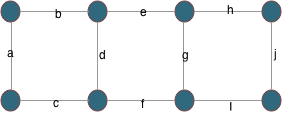
\includegraphics[scale=0.7]{img/paral.png}
}
\only<4>{
\begin{figure}[!ht]
    \centering

  \end{figure}
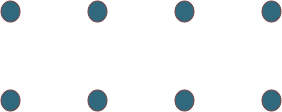
\includegraphics[scale=0.7]{img/paral1.png}
}
\only<5>{
\begin{figure}[!ht]
    \centering
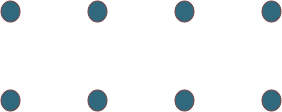
\includegraphics[scale=0.6]{img/p1.png}
  \end{figure}




\includegraphics[scale=0.7]{img/pp1.png}
}
\only<6>{
\begin{figure}[!ht]
    \centering
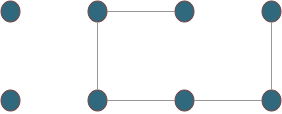
\includegraphics[scale=0.6]{img/p2.png}
  \end{figure}




\includegraphics[scale=0.7]{img/pp2.png}
}
\only<7>{
\begin{figure}[!ht]
    \centering
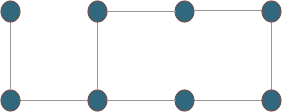
\includegraphics[scale=0.6]{img/p3.png}
  \end{figure}




\includegraphics[scale=0.7]{img/pp3.png}
}
\only<8>{
\begin{figure}[!ht]
    \centering
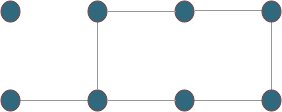
\includegraphics[scale=0.6]{img/p4.png}
  \end{figure}




\includegraphics[scale=0.7]{img/pp4.png}
}

\end{frame}

\begin{frame}
  \frametitle{Getting Random Number at $O(1)$}
\only<1>{
There will be multi edges, and suppose we give multiedges at random
edge a score chosen randomly from
interval [0, k]. The probability distribution for the minimum score X
among $wk$ edges:
$$Pr[X > t] = (1 - t/k)^{wk}$$

and when $k$ grows bigger:
$$Pr[x > t] = E^{-wt}$$

}

\only<2>{

  \begin{itemize}
  \item Contraction algorithms can be implemented RNC using $m$
    processors on an m edge.
  \item $$O(n^2)$$ Processors for minimum cut problems.
  \end{itemize}

}

\only<3>{
In $\log^{O(1)}{m}$ time per edge, it is possible to assign each edge
an exponentially distributed score that, with high probability, yields
the same result as COMPACT.
}


\only<4>{
  \begin{block}{Permutation(A little bit about the engineeringd
      detail)}

    \begin{itemize}


\item Setting $X = -(\ln{U})/w$
\item Selecting an integer $M = n^{O(1)}$
\item Uniformly select integers from $[1, M]$ using $O(\log{n})$ bits
\item Devide selected integer by $M$, which is uniform in $U$.
    \end{itemize}
  \end{block}
}
\only<5>{
  \begin{block}{Logrithm}
Using the first  $O(\log{n})$ terms of Taylor expansian of natural
logarithm to compute an approximation to $\ln{U}$
  \end{block}
}


\end{frame}
